% !TEX root = ../thesis.tex

\chapter{Hintergrund}

\paragraph{Ausblick:}
Zum besseren Verständnis der weiteren Verlaufs dieser Arbeit, dient dieses Kapitel zur Einführung in die zugrundeliegenden Themen. Dazu wird zunächst die featurebasierte Softwareentwicklung erläutert, ehe dann der Themenbereich des Machine Learnings vorgestellt wird. Dazu werden die Klassifikation und die Fehlervorhersage mittels Machine Learning erläutert. Unterstützt werden die Abschnitte von Grafiken zum besseren Verständnis der Zusammenhänge.
\\
\hrule

\section{Featurebasierte Softwareentwicklung}

\section{Machine-Learning-Klassifikation}

\begin{figure}[H]
    \centering
    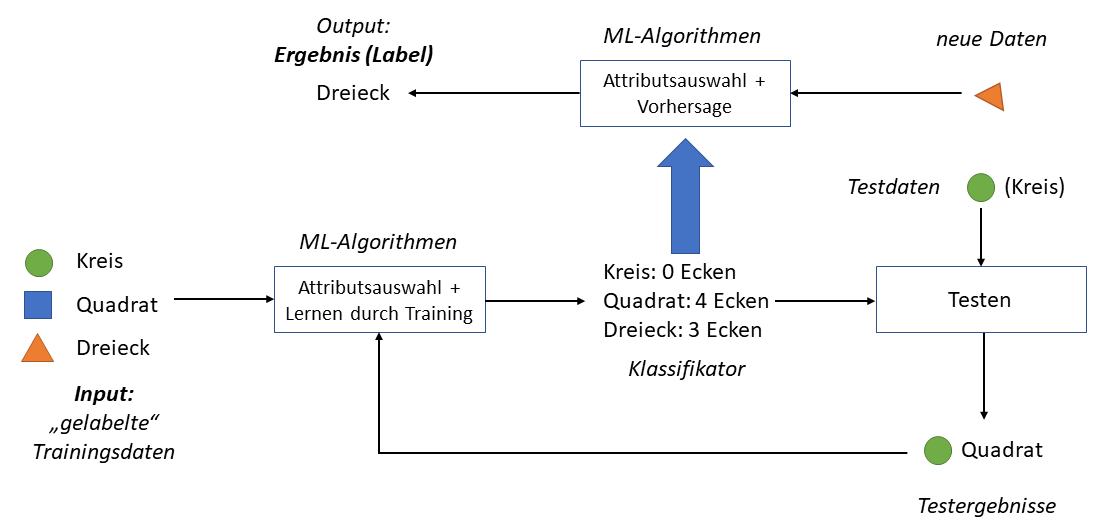
\includegraphics[width=\textwidth]{images/ML}
    \caption{Allgemeiner Prozess des überwachten Machine Learnings}\label{fig:ml}
\end{figure}

\begin{figure}[H]
    \centering
    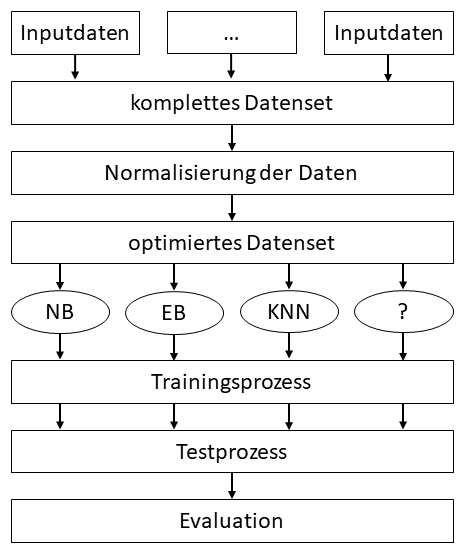
\includegraphics[width=\textwidth]{images/Prozess}
    \caption{Angewendeter Prozess zur Durchführung der Klassfikation nach \cite{Ceylan2006}}\label{fig:process}
\end{figure}

\section{Fehlervorhersage mittels Machine Learning}

\cleardoublepage
